\documentclass[1p]{elsarticle_modified}
%\bibliographystyle{elsarticle-num}

%\usepackage[colorlinks]{hyperref}
%\usepackage{abbrmath_seonhwa} %\Abb, \Ascr, \Acal ,\Abf, \Afrak
\usepackage{amsfonts}
\usepackage{amssymb}
\usepackage{amsmath}
\usepackage{amsthm}
\usepackage{scalefnt}
\usepackage{amsbsy}
\usepackage{kotex}
\usepackage{caption}
\usepackage{subfig}
\usepackage{color}
\usepackage{graphicx}
\usepackage{xcolor} %% white, black, red, green, blue, cyan, magenta, yellow
\usepackage{float}
\usepackage{setspace}
\usepackage{hyperref}

\usepackage{tikz}
\usetikzlibrary{arrows}

\usepackage{multirow}
\usepackage{array} % fixed length table
\usepackage{hhline}

%%%%%%%%%%%%%%%%%%%%%
\makeatletter
\renewcommand*\env@matrix[1][\arraystretch]{%
	\edef\arraystretch{#1}%
	\hskip -\arraycolsep
	\let\@ifnextchar\new@ifnextchar
	\array{*\c@MaxMatrixCols c}}
\makeatother %https://tex.stackexchange.com/questions/14071/how-can-i-increase-the-line-spacing-in-a-matrix
%%%%%%%%%%%%%%%

\usepackage[normalem]{ulem}

\newcommand{\msout}[1]{\ifmmode\text{\sout{\ensuremath{#1}}}\else\sout{#1}\fi}
%SOURCE: \msout is \stkout macro in https://tex.stackexchange.com/questions/20609/strikeout-in-math-mode

\newcommand{\cancel}[1]{
	\ifmmode
	{\color{red}\msout{#1}}
	\else
	{\color{red}\sout{#1}}
	\fi
}

\newcommand{\add}[1]{
	{\color{blue}\uwave{#1}}
}

\newcommand{\replace}[2]{
	\ifmmode
	{\color{red}\msout{#1}}{\color{blue}\uwave{#2}}
	\else
	{\color{red}\sout{#1}}{\color{blue}\uwave{#2}}
	\fi
}

\newcommand{\Sol}{\mathcal{S}} %segment
\newcommand{\D}{D} %diagram
\newcommand{\A}{\mathcal{A}} %arc


%%%%%%%%%%%%%%%%%%%%%%%%%%%%%5 test

\def\sl{\operatorname{\textup{SL}}(2,\Cbb)}
\def\psl{\operatorname{\textup{PSL}}(2,\Cbb)}
\def\quan{\mkern 1mu \triangleright \mkern 1mu}

\theoremstyle{definition}
\newtheorem{thm}{Theorem}[section]
\newtheorem{prop}[thm]{Proposition}
\newtheorem{lem}[thm]{Lemma}
\newtheorem{ques}[thm]{Question}
\newtheorem{cor}[thm]{Corollary}
\newtheorem{defn}[thm]{Definition}
\newtheorem{exam}[thm]{Example}
\newtheorem{rmk}[thm]{Remark}
\newtheorem{alg}[thm]{Algorithm}

\newcommand{\I}{\sqrt{-1}}
\begin{document}

%\begin{frontmatter}
%
%\title{Boundary parabolic representations of knots up to 8 crossings}
%
%%% Group authors per affiliation:
%\author{Yunhi Cho} 
%\address{Department of Mathematics, University of Seoul, Seoul, Korea}
%\ead{yhcho@uos.ac.kr}
%
%
%\author{Seonhwa Kim} %\fnref{s_kim}}
%\address{Center for Geometry and Physics, Institute for Basic Science, Pohang, 37673, Korea}
%\ead{ryeona17@ibs.re.kr}
%
%\author{Hyuk Kim}
%\address{Department of Mathematical Sciences, Seoul National University, Seoul 08826, Korea}
%\ead{hyukkim@snu.ac.kr}
%
%\author{Seokbeom Yoon}
%\address{Department of Mathematical Sciences, Seoul National University, Seoul, 08826,  Korea}
%\ead{sbyoon15@snu.ac.kr}
%
%\begin{abstract}
%We find all boundary parabolic representation of knots up to 8 crossings.
%
%\end{abstract}
%\begin{keyword}
%    \MSC[2010] 57M25 
%\end{keyword}
%
%\end{frontmatter}

%\linenumbers
%\tableofcontents
%
\newcommand\colored[1]{\textcolor{white}{\rule[-0.35ex]{0.8em}{1.4ex}}\kern-0.8em\color{red} #1}%
%\newcommand\colored[1]{\textcolor{white}{ #1}\kern-2.17ex	\textcolor{white}{ #1}\kern-1.81ex	\textcolor{white}{ #1}\kern-2.15ex\color{red}#1	}

{\Large $\underline{12a_{1044}~(K12a_{1044})}$}

\setlength{\tabcolsep}{10pt}
\renewcommand{\arraystretch}{1.6}
\vspace{1cm}\begin{tabular}{m{100pt}>{\centering\arraybackslash}m{274pt}}
\multirow{5}{120pt}{
	\centering
	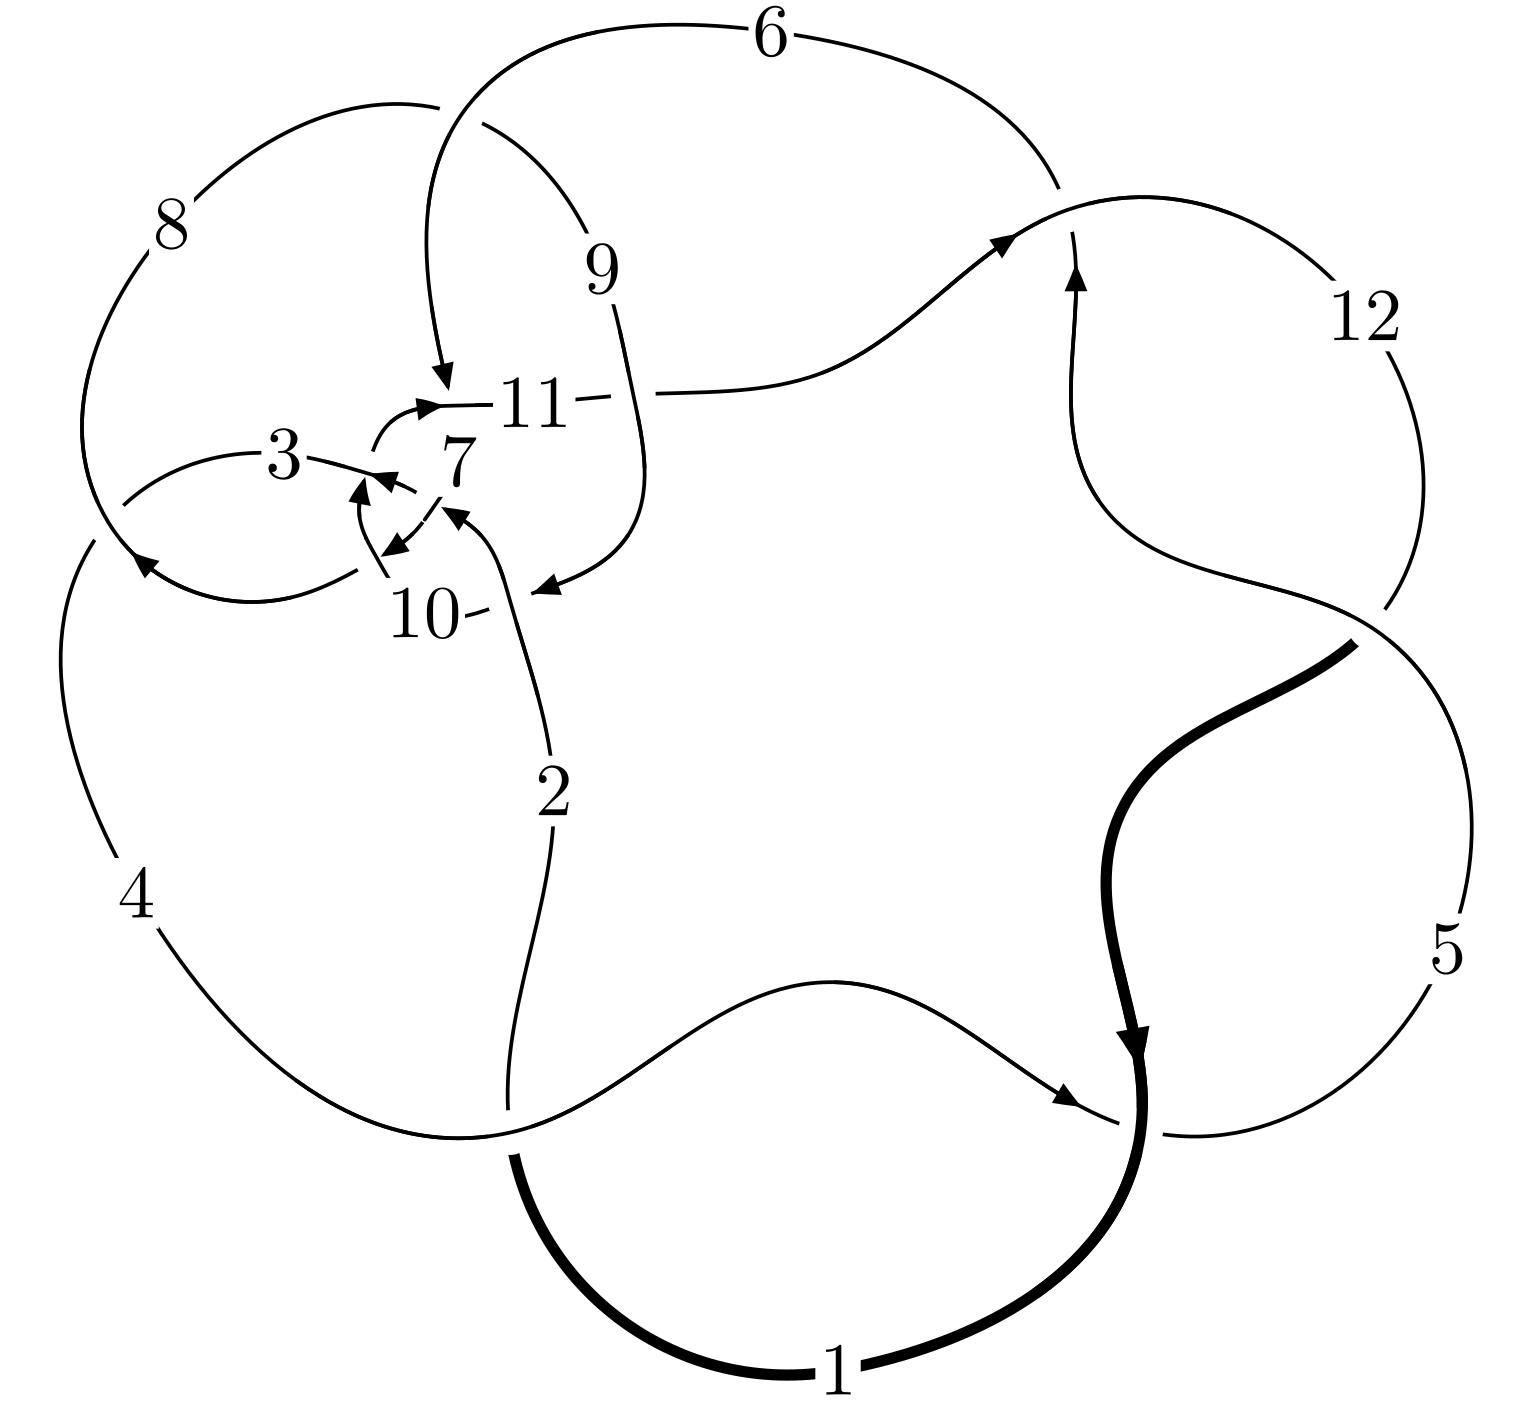
\includegraphics[width=112pt]{../../../GIT/diagram.site/Diagrams/png/1845_12a_1044.png}\\
\ \ \ A knot diagram\footnotemark}&
\allowdisplaybreaks
\textbf{Linearized knot diagam} \\
\cline{2-2}
 &
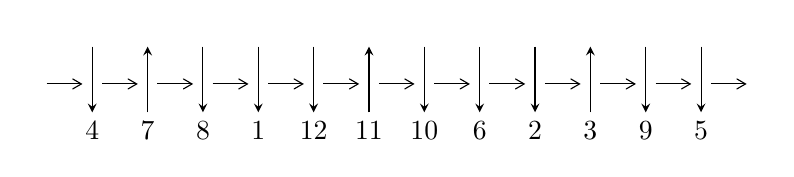
\begin{tikzpicture}[x=20pt, y=17pt]
	% nodes
	\node (C0) at (0, 0) {};
	\node (C1) at (1, 0) {};
	\node (C1U) at (1, +1) {};
	\node (C1D) at (1, -1) {4};

	\node (C2) at (2, 0) {};
	\node (C2U) at (2, +1) {};
	\node (C2D) at (2, -1) {7};

	\node (C3) at (3, 0) {};
	\node (C3U) at (3, +1) {};
	\node (C3D) at (3, -1) {8};

	\node (C4) at (4, 0) {};
	\node (C4U) at (4, +1) {};
	\node (C4D) at (4, -1) {1};

	\node (C5) at (5, 0) {};
	\node (C5U) at (5, +1) {};
	\node (C5D) at (5, -1) {12};

	\node (C6) at (6, 0) {};
	\node (C6U) at (6, +1) {};
	\node (C6D) at (6, -1) {11};

	\node (C7) at (7, 0) {};
	\node (C7U) at (7, +1) {};
	\node (C7D) at (7, -1) {10};

	\node (C8) at (8, 0) {};
	\node (C8U) at (8, +1) {};
	\node (C8D) at (8, -1) {6};

	\node (C9) at (9, 0) {};
	\node (C9U) at (9, +1) {};
	\node (C9D) at (9, -1) {2};

	\node (C10) at (10, 0) {};
	\node (C10U) at (10, +1) {};
	\node (C10D) at (10, -1) {3};

	\node (C11) at (11, 0) {};
	\node (C11U) at (11, +1) {};
	\node (C11D) at (11, -1) {9};

	\node (C12) at (12, 0) {};
	\node (C12U) at (12, +1) {};
	\node (C12D) at (12, -1) {5};
	\node (C13) at (13, 0) {};

	% arrows
	\draw[->,>={angle 60}]
	(C0) edge (C1) (C1) edge (C2) (C2) edge (C3) (C3) edge (C4) (C4) edge (C5) (C5) edge (C6) (C6) edge (C7) (C7) edge (C8) (C8) edge (C9) (C9) edge (C10) (C10) edge (C11) (C11) edge (C12) (C12) edge (C13) ;	\draw[->,>=stealth]
	(C1U) edge (C1D) (C2D) edge (C2U) (C3U) edge (C3D) (C4U) edge (C4D) (C5U) edge (C5D) (C6D) edge (C6U) (C7U) edge (C7D) (C8U) edge (C8D) (C9U) edge (C9D) (C10D) edge (C10U) (C11U) edge (C11D) (C12U) edge (C12D) ;
	\end{tikzpicture} \\
\hhline{~~} \\& 
\textbf{Solving Sequence} \\ \cline{2-2} 
 &
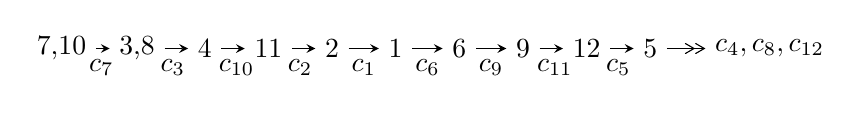
\begin{tikzpicture}[x=23pt, y=7pt]
	% node
	\node (A0) at (-1/8, 0) {7,10};
	\node (A1) at (17/16, 0) {3,8};
	\node (A2) at (17/8, 0) {4};
	\node (A3) at (25/8, 0) {11};
	\node (A4) at (33/8, 0) {2};
	\node (A5) at (41/8, 0) {1};
	\node (A6) at (49/8, 0) {6};
	\node (A7) at (57/8, 0) {9};
	\node (A8) at (65/8, 0) {12};
	\node (A9) at (73/8, 0) {5};
	\node (C1) at (1/2, -1) {$c_{7}$};
	\node (C2) at (13/8, -1) {$c_{3}$};
	\node (C3) at (21/8, -1) {$c_{10}$};
	\node (C4) at (29/8, -1) {$c_{2}$};
	\node (C5) at (37/8, -1) {$c_{1}$};
	\node (C6) at (45/8, -1) {$c_{6}$};
	\node (C7) at (53/8, -1) {$c_{9}$};
	\node (C8) at (61/8, -1) {$c_{11}$};
	\node (C9) at (69/8, -1) {$c_{5}$};
	\node (A10) at (11, 0) {$c_{4},c_{8},c_{12}$};

	% edge
	\draw[->,>=stealth]	
	(A0) edge (A1) (A1) edge (A2) (A2) edge (A3) (A3) edge (A4) (A4) edge (A5) (A5) edge (A6) (A6) edge (A7) (A7) edge (A8) (A8) edge (A9) ;
	\draw[->>,>={angle 60}]	
	(A9) edge (A10);
\end{tikzpicture} \\ 

\end{tabular} \\

\footnotetext{
The image of knot diagram is generated by the software ``\textbf{Draw programme}" developed by Andrew Bartholomew(\url{http://www.layer8.co.uk/maths/draw/index.htm\#Running-draw}), where we modified some parts for our purpose(\url{https://github.com/CATsTAILs/LinksPainter}).
}\phantom \\ \newline 
\centering \textbf{Ideals for irreducible components\footnotemark of $X_{\text{par}}$} 
 
\begin{align*}
I^u_{1}&=\langle 
-9.07361\times10^{36} u^{42}-2.49991\times10^{38} u^{41}+\cdots+3.01538\times10^{35} b+8.06957\times10^{37},\\
\phantom{I^u_{1}}&\phantom{= \langle  }-4.03479\times10^{37} u^{42}-1.11159\times10^{39} u^{41}+\cdots+6.03076\times10^{35} a+3.58061\times10^{38},\\
\phantom{I^u_{1}}&\phantom{= \langle  }u^{43}+28 u^{42}+\cdots-18 u-4\rangle \\
I^u_{2}&=\langle 
-6967 u^{18} a^3-29606 u^{18} a^2+\cdots-20917 a+13395,\;u^{18} a^3+9 u^{18} a^2+\cdots+15 a^2+25,\\
\phantom{I^u_{2}}&\phantom{= \langle  }u^{19}-9 u^{18}+\cdots-5 u^2+1\rangle \\
I^u_{3}&=\langle 
300258 u^{21}-3737558 u^{20}+\cdots+83731 b-586404,\\
\phantom{I^u_{3}}&\phantom{= \langle  }586404 u^{21}-7322994 u^{20}+\cdots+83731 a-1066330,\;u^{22}-13 u^{21}+\cdots-5 u+1\rangle \\
\\
\end{align*}
\raggedright * 3 irreducible components of $\dim_{\mathbb{C}}=0$, with total 141 representations.\\
\footnotetext{All coefficients of polynomials are rational numbers. But the coefficients are sometimes approximated in decimal forms when there is not enough margin.}
\newpage
\renewcommand{\arraystretch}{1}
\centering \section*{I. $I^u_{1}= \langle -9.07\times10^{36} u^{42}-2.50\times10^{38} u^{41}+\cdots+3.02\times10^{35} b+8.07\times10^{37},\;-4.03\times10^{37} u^{42}-1.11\times10^{39} u^{41}+\cdots+6.03\times10^{35} a+3.58\times10^{38},\;u^{43}+28 u^{42}+\cdots-18 u-4 \rangle$}
\flushleft \textbf{(i) Arc colorings}\\
\begin{tabular}{m{7pt} m{180pt} m{7pt} m{180pt} }
\flushright $a_{7}=$&$\begin{pmatrix}1\\0\end{pmatrix}$ \\
\flushright $a_{10}=$&$\begin{pmatrix}0\\u\end{pmatrix}$ \\
\flushright $a_{3}=$&$\begin{pmatrix}66.9034 u^{42}+1843.21 u^{41}+\cdots-1350.13 u-593.724\\30.0911 u^{42}+829.054 u^{41}+\cdots-610.538 u-267.614\end{pmatrix}$ \\
\flushright $a_{8}=$&$\begin{pmatrix}1\\u^2\end{pmatrix}$ \\
\flushright $a_{4}=$&$\begin{pmatrix}50.3090 u^{42}+1386.73 u^{41}+\cdots-1013.61 u-446.475\\25.2456 u^{42}+696.395 u^{41}+\cdots-529.788 u-234.919\end{pmatrix}$ \\
\flushright $a_{11}=$&$\begin{pmatrix}-98.4362 u^{42}-2711.47 u^{41}+\cdots+2005.14 u+868.683\\-44.7454 u^{42}-1232.43 u^{41}+\cdots+904.168 u+393.745\end{pmatrix}$ \\
\flushright $a_{2}=$&$\begin{pmatrix}36.8123 u^{42}+1014.15 u^{41}+\cdots-739.587 u-326.111\\30.0911 u^{42}+829.054 u^{41}+\cdots-610.538 u-267.614\end{pmatrix}$ \\
\flushright $a_{1}=$&$\begin{pmatrix}73.3891 u^{42}+2021.12 u^{41}+\cdots-1468.02 u-641.215\\49.4695 u^{42}+1362.87 u^{41}+\cdots-1004.50 u-437.492\end{pmatrix}$ \\
\flushright $a_{6}=$&$\begin{pmatrix}68.7543 u^{42}+1894.58 u^{41}+\cdots-1384.29 u-631.191\\50.9823 u^{42}+1403.48 u^{41}+\cdots-1017.06 u-453.999\end{pmatrix}$ \\
\flushright $a_{9}=$&$\begin{pmatrix}-29.3850 u^{42}-809.446 u^{41}+\cdots+610.479 u+260.175\\-24.3059 u^{42}-669.592 u^{41}+\cdots+492.496 u+214.763\end{pmatrix}$ \\
\flushright $a_{12}=$&$\begin{pmatrix}-96.7826 u^{42}-2666.41 u^{41}+\cdots+1954.20 u+856.576\\-58.6162 u^{42}-1614.92 u^{41}+\cdots+1190.66 u+525.323\end{pmatrix}$ \\
\flushright $a_{5}=$&$\begin{pmatrix}65.9599 u^{42}+1818.07 u^{41}+\cdots-1334.13 u-599.264\\42.8407 u^{42}+1180.03 u^{41}+\cdots-866.574 u-384.197\end{pmatrix}$\\&\end{tabular}
\flushleft \textbf{(ii) Obstruction class $= -1$}\\~\\
\flushleft \textbf{(iii) Cusp Shapes $= -119.862 u^{42}-3311.57 u^{41}+\cdots+2522.42 u+1244.58$}\\~\\
\newpage\renewcommand{\arraystretch}{1}
\flushleft \textbf{(iv) u-Polynomials at the component}\newline \\
\begin{tabular}{m{50pt}|m{274pt}}
Crossings & \hspace{64pt}u-Polynomials at each crossing \\
\hline $$\begin{aligned}c_{1},c_{4},c_{5}\\c_{12}\end{aligned}$$&$\begin{aligned}
&u^{43}-9 u^{42}+\cdots-172 u+16
\end{aligned}$\\
\hline $$\begin{aligned}c_{2},c_{10}\end{aligned}$$&$\begin{aligned}
&u^{43}-2 u^{41}+\cdots-2 u+1
\end{aligned}$\\
\hline $$\begin{aligned}c_{3},c_{9}\end{aligned}$$&$\begin{aligned}
&u^{43}- u^{42}+\cdots-16 u+2
\end{aligned}$\\
\hline $$\begin{aligned}c_{6}\end{aligned}$$&$\begin{aligned}
&u^{43}-32 u^{42}+\cdots-7864320 u+524288
\end{aligned}$\\
\hline $$\begin{aligned}c_{7}\end{aligned}$$&$\begin{aligned}
&u^{43}-28 u^{42}+\cdots-18 u+4
\end{aligned}$\\
\hline $$\begin{aligned}c_{8},c_{11}\end{aligned}$$&$\begin{aligned}
&u^{43}+3 u^{42}+\cdots+20 u+1
\end{aligned}$\\
\hline
\end{tabular}\\~\\
\newpage\renewcommand{\arraystretch}{1}
\flushleft \textbf{(v) Riley Polynomials at the component}\newline \\
\begin{tabular}{m{50pt}|m{274pt}}
Crossings & \hspace{64pt}Riley Polynomials at each crossing \\
\hline $$\begin{aligned}c_{1},c_{4},c_{5}\\c_{12}\end{aligned}$$&$\begin{aligned}
&y^{43}+51 y^{42}+\cdots-3536 y-256
\end{aligned}$\\
\hline $$\begin{aligned}c_{2},c_{10}\end{aligned}$$&$\begin{aligned}
&y^{43}-4 y^{42}+\cdots+8 y-1
\end{aligned}$\\
\hline $$\begin{aligned}c_{3},c_{9}\end{aligned}$$&$\begin{aligned}
&y^{43}-9 y^{42}+\cdots+96 y-4
\end{aligned}$\\
\hline $$\begin{aligned}c_{6}\end{aligned}$$&$\begin{aligned}
&y^{43}+18 y^{42}+\cdots-137438953472 y-274877906944
\end{aligned}$\\
\hline $$\begin{aligned}c_{7}\end{aligned}$$&$\begin{aligned}
&y^{43}+2 y^{42}+\cdots+668 y-16
\end{aligned}$\\
\hline $$\begin{aligned}c_{8},c_{11}\end{aligned}$$&$\begin{aligned}
&y^{43}+23 y^{42}+\cdots+94 y-1
\end{aligned}$\\
\hline
\end{tabular}\\~\\
\newpage\flushleft \textbf{(vi) Complex Volumes and Cusp Shapes}
$$\begin{array}{c|c|c}  
\text{Solutions to }I^u_{1}& \I (\text{vol} + \sqrt{-1}CS) & \text{Cusp shape}\\
 \hline 
\begin{aligned}
u &= -0.619281 + 0.736910 I \\
a &= \phantom{-}0.20054 - 1.52504 I \\
b &= -0.99963 - 1.09221 I\end{aligned}
 & \phantom{-}9.96243 + 4.04675 I & \phantom{-0.000000 } 0 \\ \hline\begin{aligned}
u &= -0.619281 - 0.736910 I \\
a &= \phantom{-}0.20054 + 1.52504 I \\
b &= -0.99963 + 1.09221 I\end{aligned}
 & \phantom{-}9.96243 - 4.04675 I & \phantom{-0.000000 } 0 \\ \hline\begin{aligned}
u &= -0.593747 + 0.928986 I \\
a &= -0.031042 - 0.926856 I \\
b &= -0.879468 - 0.521481 I\end{aligned}
 & \phantom{-}5.16180 - 0.19404 I & \phantom{-0.000000 } 0 \\ \hline\begin{aligned}
u &= -0.593747 - 0.928986 I \\
a &= -0.031042 + 0.926856 I \\
b &= -0.879468 + 0.521481 I\end{aligned}
 & \phantom{-}5.16180 + 0.19404 I & \phantom{-0.000000 } 0 \\ \hline\begin{aligned}
u &= -1.228530 + 0.119928 I \\
a &= -0.547925 - 0.708005 I \\
b &= -0.758052 - 0.804094 I\end{aligned}
 & \phantom{-}7.54354 + 0.37611 I & \phantom{-0.000000 } 0 \\ \hline\begin{aligned}
u &= -1.228530 - 0.119928 I \\
a &= -0.547925 + 0.708005 I \\
b &= -0.758052 + 0.804094 I\end{aligned}
 & \phantom{-}7.54354 - 0.37611 I & \phantom{-0.000000 } 0 \\ \hline\begin{aligned}
u &= -0.975794 + 0.782038 I \\
a &= \phantom{-}0.076356 + 1.241860 I \\
b &= \phantom{-}1.04569 + 1.15208 I\end{aligned}
 & -0.28345 + 6.38071 I & \phantom{-0.000000 } 0 \\ \hline\begin{aligned}
u &= -0.975794 - 0.782038 I \\
a &= \phantom{-}0.076356 - 1.241860 I \\
b &= \phantom{-}1.04569 - 1.15208 I\end{aligned}
 & -0.28345 - 6.38071 I & \phantom{-0.000000 } 0 \\ \hline\begin{aligned}
u &= -0.507092 + 1.162540 I \\
a &= -0.081421 + 0.837209 I \\
b &= \phantom{-}0.932000 + 0.519197 I\end{aligned}
 & \phantom{-}13.99450 - 1.63545 I & \phantom{-0.000000 } 0 \\ \hline\begin{aligned}
u &= -0.507092 - 1.162540 I \\
a &= -0.081421 - 0.837209 I \\
b &= \phantom{-}0.932000 - 0.519197 I\end{aligned}
 & \phantom{-}13.99450 + 1.63545 I & \phantom{-0.000000 } 0\\
 \hline 
 \end{array}$$\newpage$$\begin{array}{c|c|c}  
\text{Solutions to }I^u_{1}& \I (\text{vol} + \sqrt{-1}CS) & \text{Cusp shape}\\
 \hline 
\begin{aligned}
u &= -1.069420 + 0.710868 I \\
a &= \phantom{-}0.324200 + 0.759138 I \\
b &= \phantom{-}0.886353 + 0.581374 I\end{aligned}
 & \phantom{-}1.42612 + 2.66485 I & \phantom{-0.000000 } 0 \\ \hline\begin{aligned}
u &= -1.069420 - 0.710868 I \\
a &= \phantom{-}0.324200 - 0.759138 I \\
b &= \phantom{-}0.886353 - 0.581374 I\end{aligned}
 & \phantom{-}1.42612 - 2.66485 I & \phantom{-0.000000 } 0 \\ \hline\begin{aligned}
u &= \phantom{-}0.687050\phantom{ +0.000000I} \\
a &= \phantom{-}0.599117\phantom{ +0.000000I} \\
b &= -0.411623\phantom{ +0.000000I}\end{aligned}
 & -1.10828\phantom{ +0.000000I} & -9.43920\phantom{ +0.000000I} \\ \hline\begin{aligned}
u &= \phantom{-}0.336275 + 0.564768 I \\
a &= \phantom{-}0.699167 - 1.217530 I \\
b &= -0.922733 + 0.014557 I\end{aligned}
 & \phantom{-}9.44828 - 2.46853 I & \phantom{-}1.53023 + 3.59562 I \\ \hline\begin{aligned}
u &= \phantom{-}0.336275 - 0.564768 I \\
a &= \phantom{-}0.699167 + 1.217530 I \\
b &= -0.922733 - 0.014557 I\end{aligned}
 & \phantom{-}9.44828 + 2.46853 I & \phantom{-}1.53023 - 3.59562 I \\ \hline\begin{aligned}
u &= -0.528719 + 0.200325 I \\
a &= \phantom{-}0.00069 + 2.22752 I \\
b &= \phantom{-}0.446594 + 1.177590 I\end{aligned}
 & -0.62097 + 2.44438 I & -15.0343 - 15.0278 I \\ \hline\begin{aligned}
u &= -0.528719 - 0.200325 I \\
a &= \phantom{-}0.00069 - 2.22752 I \\
b &= \phantom{-}0.446594 - 1.177590 I\end{aligned}
 & -0.62097 - 2.44438 I & -15.0343 + 15.0278 I \\ \hline\begin{aligned}
u &= -1.09557 + 0.93019 I \\
a &= -0.029411 - 1.088810 I \\
b &= -1.04502 - 1.16551 I\end{aligned}
 & -3.62136 + 10.95930 I & \phantom{-0.000000 } 0 \\ \hline\begin{aligned}
u &= -1.09557 - 0.93019 I \\
a &= -0.029411 + 1.088810 I \\
b &= -1.04502 + 1.16551 I\end{aligned}
 & -3.62136 - 10.95930 I & \phantom{-0.000000 } 0 \\ \hline\begin{aligned}
u &= \phantom{-}0.223350 + 0.508490 I \\
a &= -0.358014 + 1.243700 I \\
b &= \phantom{-}0.712370 - 0.095733 I\end{aligned}
 & \phantom{-}1.36482 - 1.89009 I & \phantom{-}0.58099 + 5.23171 I\\
 \hline 
 \end{array}$$\newpage$$\begin{array}{c|c|c}  
\text{Solutions to }I^u_{1}& \I (\text{vol} + \sqrt{-1}CS) & \text{Cusp shape}\\
 \hline 
\begin{aligned}
u &= \phantom{-}0.223350 - 0.508490 I \\
a &= -0.358014 - 1.243700 I \\
b &= \phantom{-}0.712370 + 0.095733 I\end{aligned}
 & \phantom{-}1.36482 + 1.89009 I & \phantom{-}0.58099 - 5.23171 I \\ \hline\begin{aligned}
u &= -1.11997 + 1.04983 I \\
a &= -0.025975 + 1.031520 I \\
b &= \phantom{-}1.05383 + 1.18254 I\end{aligned}
 & -1.2574 + 15.5298 I & \phantom{-0.000000 } 0 \\ \hline\begin{aligned}
u &= -1.11997 - 1.04983 I \\
a &= -0.025975 - 1.031520 I \\
b &= \phantom{-}1.05383 - 1.18254 I\end{aligned}
 & -1.2574 - 15.5298 I & \phantom{-0.000000 } 0 \\ \hline\begin{aligned}
u &= -0.443394 + 0.008368 I \\
a &= \phantom{-}1.66096 - 1.26229 I \\
b &= \phantom{-}0.725895 - 0.573592 I\end{aligned}
 & \phantom{-}0.83810 - 1.87876 I & \phantom{-}0.39664 + 2.99774 I \\ \hline\begin{aligned}
u &= -0.443394 - 0.008368 I \\
a &= \phantom{-}1.66096 + 1.26229 I \\
b &= \phantom{-}0.725895 + 0.573592 I\end{aligned}
 & \phantom{-}0.83810 + 1.87876 I & \phantom{-}0.39664 - 2.99774 I \\ \hline\begin{aligned}
u &= \phantom{-}0.351842 + 0.194871 I \\
a &= -2.94605 + 0.20344 I \\
b &= \phantom{-}1.076190 + 0.502519 I\end{aligned}
 & \phantom{-}8.75469 + 1.88268 I & -0.00595 - 3.28324 I \\ \hline\begin{aligned}
u &= \phantom{-}0.351842 - 0.194871 I \\
a &= -2.94605 - 0.20344 I \\
b &= \phantom{-}1.076190 - 0.502519 I\end{aligned}
 & \phantom{-}8.75469 - 1.88268 I & -0.00595 + 3.28324 I \\ \hline\begin{aligned}
u &= -1.12504 + 1.14203 I \\
a &= \phantom{-}0.064944 - 0.996760 I \\
b &= -1.06527 - 1.19556 I\end{aligned}
 & \phantom{-}7.3041 + 18.4273 I & \phantom{-0.000000 } 0 \\ \hline\begin{aligned}
u &= -1.12504 - 1.14203 I \\
a &= \phantom{-}0.064944 + 0.996760 I \\
b &= -1.06527 + 1.19556 I\end{aligned}
 & \phantom{-}7.3041 - 18.4273 I & \phantom{-0.000000 } 0 \\ \hline\begin{aligned}
u &= -1.28079 + 0.98206 I \\
a &= -0.218083 - 0.599042 I \\
b &= -0.867616 - 0.553074 I\end{aligned}
 & \phantom{-}2.84744 + 7.10779 I & \phantom{-0.000000 } 0\\
 \hline 
 \end{array}$$\newpage$$\begin{array}{c|c|c}  
\text{Solutions to }I^u_{1}& \I (\text{vol} + \sqrt{-1}CS) & \text{Cusp shape}\\
 \hline 
\begin{aligned}
u &= -1.28079 - 0.98206 I \\
a &= -0.218083 + 0.599042 I \\
b &= -0.867616 + 0.553074 I\end{aligned}
 & \phantom{-}2.84744 - 7.10779 I & \phantom{-0.000000 } 0 \\ \hline\begin{aligned}
u &= -0.87810 + 1.42078 I \\
a &= -0.356045 + 0.017937 I \\
b &= -0.287159 + 0.521613 I\end{aligned}
 & -2.50543 - 3.29694 I & \phantom{-0.000000 } 0 \\ \hline\begin{aligned}
u &= -0.87810 - 1.42078 I \\
a &= -0.356045 - 0.017937 I \\
b &= -0.287159 - 0.521613 I\end{aligned}
 & -2.50543 + 3.29694 I & \phantom{-0.000000 } 0 \\ \hline\begin{aligned}
u &= \phantom{-}0.183954 + 0.099778 I \\
a &= \phantom{-}5.23413 - 0.12638 I \\
b &= -0.975449 - 0.499001 I\end{aligned}
 & \phantom{-}0.95612 + 1.98935 I & \phantom{-}0.00401 - 3.39354 I \\ \hline\begin{aligned}
u &= \phantom{-}0.183954 - 0.099778 I \\
a &= \phantom{-}5.23413 + 0.12638 I \\
b &= -0.975449 + 0.499001 I\end{aligned}
 & \phantom{-}0.95612 - 1.98935 I & \phantom{-}0.00401 + 3.39354 I \\ \hline\begin{aligned}
u &= -1.34458 + 1.19695 I \\
a &= \phantom{-}0.135418 + 0.548413 I \\
b &= \phantom{-}0.838502 + 0.575295 I\end{aligned}
 & \phantom{-}10.9150 + 10.1097 I & \phantom{-0.000000 } 0 \\ \hline\begin{aligned}
u &= -1.34458 - 1.19695 I \\
a &= \phantom{-}0.135418 - 0.548413 I \\
b &= \phantom{-}0.838502 - 0.575295 I\end{aligned}
 & \phantom{-}10.9150 - 10.1097 I & \phantom{-0.000000 } 0 \\ \hline\begin{aligned}
u &= -1.31475 + 1.27295 I \\
a &= \phantom{-}0.349842 - 0.161305 I \\
b &= \phantom{-}0.254620 - 0.657408 I\end{aligned}
 & -1.00239 - 7.03044 I & \phantom{-0.000000 } 0 \\ \hline\begin{aligned}
u &= -1.31475 - 1.27295 I \\
a &= \phantom{-}0.349842 + 0.161305 I \\
b &= \phantom{-}0.254620 + 0.657408 I\end{aligned}
 & -1.00239 + 7.03044 I & \phantom{-0.000000 } 0 \\ \hline\begin{aligned}
u &= \phantom{-}0.25305 + 1.89084 I \\
a &= \phantom{-}0.123915 + 0.158134 I \\
b &= \phantom{-}0.267649 - 0.274318 I\end{aligned}
 & \phantom{-}2.16526 - 1.06347 I & \phantom{-0.000000 } 0\\
 \hline 
 \end{array}$$\newpage$$\begin{array}{c|c|c}  
\text{Solutions to }I^u_{1}& \I (\text{vol} + \sqrt{-1}CS) & \text{Cusp shape}\\
 \hline 
\begin{aligned}
u &= \phantom{-}0.25305 - 1.89084 I \\
a &= \phantom{-}0.123915 - 0.158134 I \\
b &= \phantom{-}0.267649 + 0.274318 I\end{aligned}
 & \phantom{-}2.16526 + 1.06347 I & \phantom{-0.000000 } 0 \\ \hline\begin{aligned}
u &= -1.56723 + 1.17558 I \\
a &= -0.325755 + 0.235679 I \\
b &= -0.233475 + 0.752315 I\end{aligned}
 & \phantom{-}6.94224 - 9.40178 I & \phantom{-0.000000 } 0 \\ \hline\begin{aligned}
u &= -1.56723 - 1.17558 I \\
a &= -0.325755 - 0.235679 I \\
b &= -0.233475 - 0.752315 I\end{aligned}
 & \phantom{-}6.94224 + 9.40178 I & \phantom{-0.000000 } 0\\
 \hline 
 \end{array}$$\newpage\newpage\renewcommand{\arraystretch}{1}
\centering \section*{II. $I^u_{2}= \langle -6967 a^{3} u^{18}-2.96\times10^{4} a^{2} u^{18}+\cdots-2.09\times10^{4} a+1.34\times10^{4},\;u^{18} a^3+9 u^{18} a^2+\cdots+15 a^2+25,\;u^{19}-9 u^{18}+\cdots-5 u^2+1 \rangle$}
\flushleft \textbf{(i) Arc colorings}\\
\begin{tabular}{m{7pt} m{180pt} m{7pt} m{180pt} }
\flushright $a_{7}=$&$\begin{pmatrix}1\\0\end{pmatrix}$ \\
\flushright $a_{10}=$&$\begin{pmatrix}0\\u\end{pmatrix}$ \\
\flushright $a_{3}=$&$\begin{pmatrix}a\\0.333078 a^{3} u^{18}+1.41540 a^{2} u^{18}+\cdots+a-0.640388\end{pmatrix}$ \\
\flushright $a_{8}=$&$\begin{pmatrix}1\\u^2\end{pmatrix}$ \\
\flushright $a_{4}=$&$\begin{pmatrix}-0.333078 a^{3} u^{18}-1.41540 a^{2} u^{18}+\cdots+1.70770 a^{2}+0.640388\\1.00076 a^{3} u^{18}+1.75379 a^{2} u^{18}+\cdots+a-0.0788354\end{pmatrix}$ \\
\flushright $a_{11}=$&$\begin{pmatrix}a^2 u\\-0.584596 a^{3} u^{18}-0.333078 a^{2} u^{18}+\cdots+a+0.999952\end{pmatrix}$ \\
\flushright $a_{2}=$&$\begin{pmatrix}-0.333078 a^{3} u^{18}-1.41540 a^{2} u^{18}+\cdots+1.70770 a^{2}+0.640388\\0.333078 a^{3} u^{18}+1.41540 a^{2} u^{18}+\cdots+a-0.640388\end{pmatrix}$ \\
\flushright $a_{1}=$&$\begin{pmatrix}-0.668451 a^{3} u^{18}-1.09217 a^{2} u^{18}+\cdots-a-0.482717\\0.326959 a^{3} u^{18}+1.38509 a^{2} u^{18}+\cdots+3 a-0.00970502\end{pmatrix}$ \\
\flushright $a_{6}=$&$\begin{pmatrix}0.292298 a^{3} u^{18}-0.333461 a^{2} u^{18}+\cdots-2 a+0.500024\\-0.584596 a^{3} u^{18}-0.333078 a^{2} u^{18}+\cdots+a-0.0000478080\end{pmatrix}$ \\
\flushright $a_{9}=$&$\begin{pmatrix}0.661615 a^{3} u^{18}+0.667687 a^{2} u^{18}+\cdots+2 a-0.000191232\\-0.0770187 a^{3} u^{18}-0.334608 a^{2} u^{18}+\cdots-3 a-0.999761\end{pmatrix}$ \\
\flushright $a_{12}=$&$\begin{pmatrix}0.784721 a^{3} u^{18}+0.668069 a^{2} u^{18}+\cdots+a+0.499737\\-0.246211 a^{3} u^{18}-1.00076 a^{2} u^{18}+\cdots-4 a+0.000143424\end{pmatrix}$ \\
\flushright $a_{5}=$&$\begin{pmatrix}0.0145336 a^{3} u^{18}-0.678013 a^{2} u^{18}+\cdots-a+0.502127\\0.385093 a^{3} u^{18}+0.673041 a^{2} u^{18}+\cdots+a-0.00119520\end{pmatrix}$\\&\end{tabular}
\flushleft \textbf{(ii) Obstruction class $= -1$}\\~\\
\flushleft \textbf{(iii) Cusp Shapes $= \frac{48912}{20917} u^{18} a^3+\frac{27868}{20917} u^{18} a^2+\cdots-4 a-\frac{711174}{20917}$}\\~\\
\newpage\renewcommand{\arraystretch}{1}
\flushleft \textbf{(iv) u-Polynomials at the component}\newline \\
\begin{tabular}{m{50pt}|m{274pt}}
Crossings & \hspace{64pt}u-Polynomials at each crossing \\
\hline $$\begin{aligned}c_{1},c_{4},c_{5}\\c_{12}\end{aligned}$$&$\begin{aligned}
&(u^{19}+3 u^{18}+\cdots+2 u+1)^{4}
\end{aligned}$\\
\hline $$\begin{aligned}c_{2},c_{10}\end{aligned}$$&$\begin{aligned}
&u^{76}+3 u^{75}+\cdots+2 u+1
\end{aligned}$\\
\hline $$\begin{aligned}c_{3},c_{9}\end{aligned}$$&$\begin{aligned}
&u^{76}+u^{75}+\cdots-44450 u+29629
\end{aligned}$\\
\hline $$\begin{aligned}c_{6}\end{aligned}$$&$\begin{aligned}
&(u^2+u+1)^{38}
\end{aligned}$\\
\hline $$\begin{aligned}c_{7}\end{aligned}$$&$\begin{aligned}
&(u^{19}+9 u^{18}+\cdots+5 u^2-1)^{4}
\end{aligned}$\\
\hline $$\begin{aligned}c_{8},c_{11}\end{aligned}$$&$\begin{aligned}
&u^{76}+u^{75}+\cdots-12 u+1
\end{aligned}$\\
\hline
\end{tabular}\\~\\
\newpage\renewcommand{\arraystretch}{1}
\flushleft \textbf{(v) Riley Polynomials at the component}\newline \\
\begin{tabular}{m{50pt}|m{274pt}}
Crossings & \hspace{64pt}Riley Polynomials at each crossing \\
\hline $$\begin{aligned}c_{1},c_{4},c_{5}\\c_{12}\end{aligned}$$&$\begin{aligned}
&(y^{19}+23 y^{18}+\cdots-10 y-1)^{4}
\end{aligned}$\\
\hline $$\begin{aligned}c_{2},c_{10}\end{aligned}$$&$\begin{aligned}
&y^{76}+27 y^{75}+\cdots+120 y+1
\end{aligned}$\\
\hline $$\begin{aligned}c_{3},c_{9}\end{aligned}$$&$\begin{aligned}
&y^{76}-17 y^{75}+\cdots-10612715258 y+877877641
\end{aligned}$\\
\hline $$\begin{aligned}c_{6}\end{aligned}$$&$\begin{aligned}
&(y^2+y+1)^{38}
\end{aligned}$\\
\hline $$\begin{aligned}c_{7}\end{aligned}$$&$\begin{aligned}
&(y^{19}- y^{18}+\cdots+10 y-1)^{4}
\end{aligned}$\\
\hline $$\begin{aligned}c_{8},c_{11}\end{aligned}$$&$\begin{aligned}
&y^{76}-9 y^{75}+\cdots-56 y+1
\end{aligned}$\\
\hline
\end{tabular}\\~\\
\newpage\flushleft \textbf{(vi) Complex Volumes and Cusp Shapes}
$$\begin{array}{c|c|c}  
\text{Solutions to }I^u_{2}& \I (\text{vol} + \sqrt{-1}CS) & \text{Cusp shape}\\
 \hline 
\begin{aligned}
u &= \phantom{-}0.224406 + 0.979990 I \\
a &= -0.079941 - 1.063040 I \\
b &= \phantom{-}0.75493 - 1.56939 I\end{aligned}
 & \phantom{-}10.77910 - 7.75317 I & \phantom{-}2.36068 + 8.39109 I \\ \hline\begin{aligned}
u &= \phantom{-}0.224406 + 0.979990 I \\
a &= -0.531501 - 1.301450 I \\
b &= \phantom{-}0.205893 + 0.046196 I\end{aligned}
 & \phantom{-}10.77910 - 3.69340 I & \phantom{-}2.36068 + 1.46289 I \\ \hline\begin{aligned}
u &= \phantom{-}0.224406 + 0.979990 I \\
a &= \phantom{-}1.35403 + 1.08041 I \\
b &= -1.023830 + 0.316893 I\end{aligned}
 & \phantom{-}10.77910 - 7.75317 I & \phantom{-}2.36068 + 8.39109 I \\ \hline\begin{aligned}
u &= \phantom{-}0.224406 + 0.979990 I \\
a &= -0.090504 + 0.189372 I \\
b &= -1.156140 + 0.812919 I\end{aligned}
 & \phantom{-}10.77910 - 3.69340 I & \phantom{-}2.36068 + 1.46289 I \\ \hline\begin{aligned}
u &= \phantom{-}0.224406 - 0.979990 I \\
a &= -0.079941 + 1.063040 I \\
b &= \phantom{-}0.75493 + 1.56939 I\end{aligned}
 & \phantom{-}10.77910 + 7.75317 I & \phantom{-}2.36068 - 8.39109 I \\ \hline\begin{aligned}
u &= \phantom{-}0.224406 - 0.979990 I \\
a &= -0.531501 + 1.301450 I \\
b &= \phantom{-}0.205893 - 0.046196 I\end{aligned}
 & \phantom{-}10.77910 + 3.69340 I & \phantom{-}2.36068 - 1.46289 I \\ \hline\begin{aligned}
u &= \phantom{-}0.224406 - 0.979990 I \\
a &= \phantom{-}1.35403 - 1.08041 I \\
b &= -1.023830 - 0.316893 I\end{aligned}
 & \phantom{-}10.77910 + 7.75317 I & \phantom{-}2.36068 - 8.39109 I \\ \hline\begin{aligned}
u &= \phantom{-}0.224406 - 0.979990 I \\
a &= -0.090504 - 0.189372 I \\
b &= -1.156140 - 0.812919 I\end{aligned}
 & \phantom{-}10.77910 + 3.69340 I & \phantom{-}2.36068 - 1.46289 I \\ \hline\begin{aligned}
u &= \phantom{-}0.411578 + 0.796293 I \\
a &= -0.017212 + 1.037780 I \\
b &= -0.87911 + 1.55841 I\end{aligned}
 & \phantom{-}1.87060 - 6.27257 I & \phantom{-}0.97656 + 11.51556 I \\ \hline\begin{aligned}
u &= \phantom{-}0.411578 + 0.796293 I \\
a &= -0.100441 + 1.281310 I \\
b &= -0.0472227 - 0.0855841 I\end{aligned}
 & \phantom{-}1.87060 - 2.21281 I & \phantom{-}0.97656 + 4.58736 I\\
 \hline 
 \end{array}$$\newpage$$\begin{array}{c|c|c}  
\text{Solutions to }I^u_{2}& \I (\text{vol} + \sqrt{-1}CS) & \text{Cusp shape}\\
 \hline 
\begin{aligned}
u &= \phantom{-}0.411578 + 0.796293 I \\
a &= \phantom{-}0.1090080 - 0.0029603 I \\
b &= \phantom{-}1.061640 - 0.447379 I\end{aligned}
 & \phantom{-}1.87060 - 2.21281 I & \phantom{-}0.97656 + 4.58736 I \\ \hline\begin{aligned}
u &= \phantom{-}0.411578 + 0.796293 I \\
a &= -1.09415 - 1.66953 I \\
b &= \phantom{-}0.833461 - 0.413422 I\end{aligned}
 & \phantom{-}1.87060 - 6.27257 I & \phantom{-}0.97656 + 11.51556 I \\ \hline\begin{aligned}
u &= \phantom{-}0.411578 - 0.796293 I \\
a &= -0.017212 - 1.037780 I \\
b &= -0.87911 - 1.55841 I\end{aligned}
 & \phantom{-}1.87060 + 6.27257 I & \phantom{-}0.97656 - 11.51556 I \\ \hline\begin{aligned}
u &= \phantom{-}0.411578 - 0.796293 I \\
a &= -0.100441 - 1.281310 I \\
b &= -0.0472227 + 0.0855841 I\end{aligned}
 & \phantom{-}1.87060 + 2.21281 I & \phantom{-}0.97656 - 4.58736 I \\ \hline\begin{aligned}
u &= \phantom{-}0.411578 - 0.796293 I \\
a &= \phantom{-}0.1090080 + 0.0029603 I \\
b &= \phantom{-}1.061640 + 0.447379 I\end{aligned}
 & \phantom{-}1.87060 + 2.21281 I & \phantom{-}0.97656 - 4.58736 I \\ \hline\begin{aligned}
u &= \phantom{-}0.411578 - 0.796293 I \\
a &= -1.09415 + 1.66953 I \\
b &= \phantom{-}0.833461 + 0.413422 I\end{aligned}
 & \phantom{-}1.87060 + 6.27257 I & \phantom{-}0.97656 - 11.51556 I \\ \hline\begin{aligned}
u &= \phantom{-}0.738136 + 0.285129 I \\
a &= \phantom{-}0.220113 - 0.805434 I \\
b &= \phantom{-}1.18836 - 1.32414 I\end{aligned}
 & -1.93123 - 3.81353 I & -12.8478 + 10.3305 I \\ \hline\begin{aligned}
u &= \phantom{-}0.738136 + 0.285129 I \\
a &= -0.298557 - 0.491122 I \\
b &= -1.164680 - 0.741015 I\end{aligned}
 & -1.93123 + 0.24623 I & -12.84779 + 3.40225 I \\ \hline\begin{aligned}
u &= \phantom{-}0.738136 + 0.285129 I \\
a &= \phantom{-}1.71044 + 0.34319 I \\
b &= \phantom{-}0.080342 + 0.447642 I\end{aligned}
 & -1.93123 + 0.24623 I & -12.84779 + 3.40225 I \\ \hline\begin{aligned}
u &= \phantom{-}0.738136 + 0.285129 I \\
a &= -0.79794 + 2.10213 I \\
b &= -0.392126 + 0.531760 I\end{aligned}
 & -1.93123 - 3.81353 I & -12.8478 + 10.3305 I\\
 \hline 
 \end{array}$$\newpage$$\begin{array}{c|c|c}  
\text{Solutions to }I^u_{2}& \I (\text{vol} + \sqrt{-1}CS) & \text{Cusp shape}\\
 \hline 
\begin{aligned}
u &= \phantom{-}0.738136 - 0.285129 I \\
a &= \phantom{-}0.220113 + 0.805434 I \\
b &= \phantom{-}1.18836 + 1.32414 I\end{aligned}
 & -1.93123 + 3.81353 I & -12.8478 - 10.3305 I \\ \hline\begin{aligned}
u &= \phantom{-}0.738136 - 0.285129 I \\
a &= -0.298557 + 0.491122 I \\
b &= -1.164680 + 0.741015 I\end{aligned}
 & -1.93123 - 0.24623 I & -12.84779 - 3.40225 I \\ \hline\begin{aligned}
u &= \phantom{-}0.738136 - 0.285129 I \\
a &= \phantom{-}1.71044 - 0.34319 I \\
b &= \phantom{-}0.080342 - 0.447642 I\end{aligned}
 & -1.93123 - 0.24623 I & -12.84779 - 3.40225 I \\ \hline\begin{aligned}
u &= \phantom{-}0.738136 - 0.285129 I \\
a &= -0.79794 - 2.10213 I \\
b &= -0.392126 - 0.531760 I\end{aligned}
 & -1.93123 + 3.81353 I & -12.8478 - 10.3305 I \\ \hline\begin{aligned}
u &= -0.578057 + 0.369314 I \\
a &= -0.093463 + 0.827692 I \\
b &= -1.61147 + 1.31105 I\end{aligned}
 & \phantom{-}8.03276 + 9.35799 I & -5.9941 - 13.3695 I \\ \hline\begin{aligned}
u &= -0.578057 + 0.369314 I \\
a &= -0.59366 - 1.69489 I \\
b &= \phantom{-}0.069383 - 1.329150 I\end{aligned}
 & \phantom{-}8.03276 + 5.29822 I & -5.99414 - 6.44128 I \\ \hline\begin{aligned}
u &= -0.578057 + 0.369314 I \\
a &= \phantom{-}1.12844 - 1.57839 I \\
b &= -0.969117 - 0.760498 I\end{aligned}
 & \phantom{-}8.03276 + 5.29822 I & -5.99414 - 6.44128 I \\ \hline\begin{aligned}
u &= -0.578057 + 0.369314 I \\
a &= -3.00868 + 0.34582 I \\
b &= \phantom{-}0.251651 + 0.512970 I\end{aligned}
 & \phantom{-}8.03276 + 9.35799 I & -5.9941 - 13.3695 I \\ \hline\begin{aligned}
u &= -0.578057 - 0.369314 I \\
a &= -0.093463 - 0.827692 I \\
b &= -1.61147 - 1.31105 I\end{aligned}
 & \phantom{-}8.03276 - 9.35799 I & -5.9941 + 13.3695 I \\ \hline\begin{aligned}
u &= -0.578057 - 0.369314 I \\
a &= -0.59366 + 1.69489 I \\
b &= \phantom{-}0.069383 + 1.329150 I\end{aligned}
 & \phantom{-}8.03276 - 5.29822 I & -5.99414 + 6.44128 I\\
 \hline 
 \end{array}$$\newpage$$\begin{array}{c|c|c}  
\text{Solutions to }I^u_{2}& \I (\text{vol} + \sqrt{-1}CS) & \text{Cusp shape}\\
 \hline 
\begin{aligned}
u &= -0.578057 - 0.369314 I \\
a &= \phantom{-}1.12844 + 1.57839 I \\
b &= -0.969117 + 0.760498 I\end{aligned}
 & \phantom{-}8.03276 - 5.29822 I & -5.99414 + 6.44128 I \\ \hline\begin{aligned}
u &= -0.578057 - 0.369314 I \\
a &= -3.00868 - 0.34582 I \\
b &= \phantom{-}0.251651 - 0.512970 I\end{aligned}
 & \phantom{-}8.03276 - 9.35799 I & -5.9941 + 13.3695 I \\ \hline\begin{aligned}
u &= \phantom{-}1.07839 + 0.92133 I \\
a &= \phantom{-}0.020594 + 1.098290 I \\
b &= -0.650210 + 1.015400 I\end{aligned}
 & -2.60244 - 4.96452 I & -11.91453 + 1.46747 I \\ \hline\begin{aligned}
u &= \phantom{-}1.07839 + 0.92133 I \\
a &= -0.116481 - 0.842068 I \\
b &= \phantom{-}0.98968 - 1.20336 I\end{aligned}
 & -2.60244 - 4.96452 I & -11.91453 + 1.46747 I \\ \hline\begin{aligned}
u &= \phantom{-}1.07839 + 0.92133 I \\
a &= \phantom{-}0.470035 + 0.385689 I \\
b &= -0.180979 + 0.648976 I\end{aligned}
 & -2.60244 - 0.90475 I & -11.91453 - 5.46074 I \\ \hline\begin{aligned}
u &= \phantom{-}1.07839 + 0.92133 I \\
a &= -0.200198 - 0.430759 I \\
b &= -0.151536 - 0.848982 I\end{aligned}
 & -2.60244 - 0.90475 I & -11.91453 - 5.46074 I \\ \hline\begin{aligned}
u &= \phantom{-}1.07839 - 0.92133 I \\
a &= \phantom{-}0.020594 - 1.098290 I \\
b &= -0.650210 - 1.015400 I\end{aligned}
 & -2.60244 + 4.96452 I & -11.91453 - 1.46747 I \\ \hline\begin{aligned}
u &= \phantom{-}1.07839 - 0.92133 I \\
a &= -0.116481 + 0.842068 I \\
b &= \phantom{-}0.98968 + 1.20336 I\end{aligned}
 & -2.60244 + 4.96452 I & -11.91453 - 1.46747 I \\ \hline\begin{aligned}
u &= \phantom{-}1.07839 - 0.92133 I \\
a &= \phantom{-}0.470035 - 0.385689 I \\
b &= -0.180979 - 0.648976 I\end{aligned}
 & -2.60244 + 0.90475 I & -11.91453 + 5.46074 I \\ \hline\begin{aligned}
u &= \phantom{-}1.07839 - 0.92133 I \\
a &= -0.200198 + 0.430759 I \\
b &= -0.151536 + 0.848982 I\end{aligned}
 & -2.60244 + 0.90475 I & -11.91453 + 5.46074 I\\
 \hline 
 \end{array}$$\newpage$$\begin{array}{c|c|c}  
\text{Solutions to }I^u_{2}& \I (\text{vol} + \sqrt{-1}CS) & \text{Cusp shape}\\
 \hline 
\begin{aligned}
u &= -0.515417 + 0.216459 I \\
a &= \phantom{-}0.136886 - 1.007060 I \\
b &= \phantom{-}1.56792 - 1.42933 I\end{aligned}
 & -0.60400 + 6.51999 I & -13.2217 - 15.7344 I \\ \hline\begin{aligned}
u &= -0.515417 + 0.216459 I \\
a &= -0.22464 + 1.91414 I \\
b &= \phantom{-}0.704217 + 1.183980 I\end{aligned}
 & -0.60400 + 2.46023 I & -13.2217 - 8.8062 I \\ \hline\begin{aligned}
u &= -0.515417 + 0.216459 I \\
a &= \phantom{-}0.34137 + 2.44050 I \\
b &= \phantom{-}0.298549 + 1.035200 I\end{aligned}
 & -0.60400 + 2.46023 I & -13.2217 - 8.8062 I \\ \hline\begin{aligned}
u &= -0.515417 + 0.216459 I \\
a &= \phantom{-}3.57597 - 1.27135 I \\
b &= -0.147434 - 0.548687 I\end{aligned}
 & -0.60400 + 6.51999 I & -13.2217 - 15.7344 I \\ \hline\begin{aligned}
u &= -0.515417 - 0.216459 I \\
a &= \phantom{-}0.136886 + 1.007060 I \\
b &= \phantom{-}1.56792 + 1.42933 I\end{aligned}
 & -0.60400 - 6.51999 I & -13.2217 + 15.7344 I \\ \hline\begin{aligned}
u &= -0.515417 - 0.216459 I \\
a &= -0.22464 - 1.91414 I \\
b &= \phantom{-}0.704217 - 1.183980 I\end{aligned}
 & -0.60400 - 2.46023 I & -13.2217 + 8.8062 I \\ \hline\begin{aligned}
u &= -0.515417 - 0.216459 I \\
a &= \phantom{-}0.34137 - 2.44050 I \\
b &= \phantom{-}0.298549 - 1.035200 I\end{aligned}
 & -0.60400 - 2.46023 I & -13.2217 + 8.8062 I \\ \hline\begin{aligned}
u &= -0.515417 - 0.216459 I \\
a &= \phantom{-}3.57597 + 1.27135 I \\
b &= -0.147434 + 0.548687 I\end{aligned}
 & -0.60400 - 6.51999 I & -13.2217 + 15.7344 I \\ \hline\begin{aligned}
u &= \phantom{-}1.28782 + 0.69169 I \\
a &= \phantom{-}0.217129 - 1.114740 I \\
b &= \phantom{-}0.426150 - 0.961228 I\end{aligned}
 & \phantom{-}3.89129 - 4.57393 I & -8.47148 + 5.29372 I \\ \hline\begin{aligned}
u &= \phantom{-}1.28782 + 0.69169 I \\
a &= -0.621576 - 0.491356 I \\
b &= \phantom{-}0.132391 - 0.683945 I\end{aligned}
 & \phantom{-}3.89129 - 0.51417 I & -8.47148 - 1.63449 I\\
 \hline 
 \end{array}$$\newpage$$\begin{array}{c|c|c}  
\text{Solutions to }I^u_{2}& \I (\text{vol} + \sqrt{-1}CS) & \text{Cusp shape}\\
 \hline 
\begin{aligned}
u &= \phantom{-}1.28782 + 0.69169 I \\
a &= \phantom{-}0.054314 + 0.717229 I \\
b &= -1.05067 + 1.28540 I\end{aligned}
 & \phantom{-}3.89129 - 4.57393 I & -8.47148 + 5.29372 I \\ \hline\begin{aligned}
u &= \phantom{-}1.28782 + 0.69169 I \\
a &= \phantom{-}0.141597 + 0.455037 I \\
b &= \phantom{-}0.460612 + 1.062710 I\end{aligned}
 & \phantom{-}3.89129 - 0.51417 I & -8.47148 - 1.63449 I \\ \hline\begin{aligned}
u &= \phantom{-}1.28782 - 0.69169 I \\
a &= \phantom{-}0.217129 + 1.114740 I \\
b &= \phantom{-}0.426150 + 0.961228 I\end{aligned}
 & \phantom{-}3.89129 + 4.57393 I & -8.47148 - 5.29372 I \\ \hline\begin{aligned}
u &= \phantom{-}1.28782 - 0.69169 I \\
a &= -0.621576 + 0.491356 I \\
b &= \phantom{-}0.132391 + 0.683945 I\end{aligned}
 & \phantom{-}3.89129 + 0.51417 I & -8.47148 + 1.63449 I \\ \hline\begin{aligned}
u &= \phantom{-}1.28782 - 0.69169 I \\
a &= \phantom{-}0.054314 - 0.717229 I \\
b &= -1.05067 - 1.28540 I\end{aligned}
 & \phantom{-}3.89129 + 4.57393 I & -8.47148 - 5.29372 I \\ \hline\begin{aligned}
u &= \phantom{-}1.28782 - 0.69169 I \\
a &= \phantom{-}0.141597 - 0.455037 I \\
b &= \phantom{-}0.460612 - 1.062710 I\end{aligned}
 & \phantom{-}3.89129 + 0.51417 I & -8.47148 + 1.63449 I \\ \hline\begin{aligned}
u &= -0.493766\phantom{ +0.000000I} \\
a &= -0.051780 + 1.334910 I \\
b &= -1.25352 + 1.55631 I\end{aligned}
 & -3.21610 + 2.02988 I & -23.6348 - 3.4641 I \\ \hline\begin{aligned}
u &= -0.493766\phantom{ +0.000000I} \\
a &= -0.051780 - 1.334910 I \\
b &= -1.25352 - 1.55631 I\end{aligned}
 & -3.21610 - 2.02988 I & -23.6348 + 3.4641 I \\ \hline\begin{aligned}
u &= -0.493766\phantom{ +0.000000I} \\
a &= -2.53869 + 3.15193 I \\
b &= -0.025567 + 0.659131 I\end{aligned}
 & -3.21610 + 2.02988 I & -23.6348 - 3.4641 I \\ \hline\begin{aligned}
u &= -0.493766\phantom{ +0.000000I} \\
a &= -2.53869 - 3.15193 I \\
b &= -0.025567 - 0.659131 I\end{aligned}
 & -3.21610 - 2.02988 I & -23.6348 + 3.4641 I\\
 \hline 
 \end{array}$$\newpage$$\begin{array}{c|c|c}  
\text{Solutions to }I^u_{2}& \I (\text{vol} + \sqrt{-1}CS) & \text{Cusp shape}\\
 \hline 
\begin{aligned}
u &= \phantom{-}1.05045 + 1.11478 I \\
a &= -0.022759 - 0.967513 I \\
b &= \phantom{-}0.674813 - 1.211630 I\end{aligned}
 & -2.00492 - 6.85219 I & -7.9642 + 14.7411 I \\ \hline\begin{aligned}
u &= \phantom{-}1.05045 + 1.11478 I \\
a &= \phantom{-}0.273568 + 0.863111 I \\
b &= -1.05466 + 1.04170 I\end{aligned}
 & -2.00492 - 6.85219 I & -7.9642 + 14.7411 I \\ \hline\begin{aligned}
u &= \phantom{-}1.05045 + 1.11478 I \\
a &= -0.412467 - 0.506564 I \\
b &= \phantom{-}0.174195 - 0.578011 I\end{aligned}
 & -2.00492 - 2.79242 I & -7.96421 + 7.81289 I \\ \hline\begin{aligned}
u &= \phantom{-}1.05045 + 1.11478 I \\
a &= \phantom{-}0.196648 + 0.341558 I \\
b &= -0.131433 + 0.991934 I\end{aligned}
 & -2.00492 - 2.79242 I & -7.96421 + 7.81289 I \\ \hline\begin{aligned}
u &= \phantom{-}1.05045 - 1.11478 I \\
a &= -0.022759 + 0.967513 I \\
b &= \phantom{-}0.674813 + 1.211630 I\end{aligned}
 & -2.00492 + 6.85219 I & -7.9642 - 14.7411 I \\ \hline\begin{aligned}
u &= \phantom{-}1.05045 - 1.11478 I \\
a &= \phantom{-}0.273568 - 0.863111 I \\
b &= -1.05466 - 1.04170 I\end{aligned}
 & -2.00492 + 6.85219 I & -7.9642 - 14.7411 I \\ \hline\begin{aligned}
u &= \phantom{-}1.05045 - 1.11478 I \\
a &= -0.412467 + 0.506564 I \\
b &= \phantom{-}0.174195 + 0.578011 I\end{aligned}
 & -2.00492 + 2.79242 I & -7.96421 - 7.81289 I \\ \hline\begin{aligned}
u &= \phantom{-}1.05045 - 1.11478 I \\
a &= \phantom{-}0.196648 - 0.341558 I \\
b &= -0.131433 - 0.991934 I\end{aligned}
 & -2.00492 + 2.79242 I & -7.96421 - 7.81289 I \\ \hline\begin{aligned}
u &= \phantom{-}1.04957 + 1.25847 I \\
a &= \phantom{-}0.013720 + 0.933343 I \\
b &= -0.63265 + 1.28758 I\end{aligned}
 & \phantom{-}5.56101 - 7.78064 I & -5.10596 + 10.77370 I \\ \hline\begin{aligned}
u &= \phantom{-}1.04957 + 1.25847 I \\
a &= -0.356143 - 0.799738 I \\
b &= \phantom{-}1.16018 - 0.99688 I\end{aligned}
 & \phantom{-}5.56101 - 7.78064 I & -5.10596 + 10.77370 I\\
 \hline 
 \end{array}$$\newpage$$\begin{array}{c|c|c}  
\text{Solutions to }I^u_{2}& \I (\text{vol} + \sqrt{-1}CS) & \text{Cusp shape}\\
 \hline 
\begin{aligned}
u &= \phantom{-}1.04957 + 1.25847 I \\
a &= \phantom{-}0.442870 + 0.549940 I \\
b &= -0.239273 + 0.532330 I\end{aligned}
 & \phantom{-}5.56101 - 3.72087 I & -5.10596 + 3.84550 I \\ \hline\begin{aligned}
u &= \phantom{-}1.04957 + 1.25847 I \\
a &= -0.155952 - 0.320196 I \\
b &= \phantom{-}0.227258 - 1.134540 I\end{aligned}
 & \phantom{-}5.56101 - 3.72087 I & -5.10596 + 3.84550 I \\ \hline\begin{aligned}
u &= \phantom{-}1.04957 - 1.25847 I \\
a &= \phantom{-}0.013720 - 0.933343 I \\
b &= -0.63265 - 1.28758 I\end{aligned}
 & \phantom{-}5.56101 + 7.78064 I & -5.10596 - 10.77370 I \\ \hline\begin{aligned}
u &= \phantom{-}1.04957 - 1.25847 I \\
a &= -0.356143 + 0.799738 I \\
b &= \phantom{-}1.16018 + 0.99688 I\end{aligned}
 & \phantom{-}5.56101 + 7.78064 I & -5.10596 - 10.77370 I \\ \hline\begin{aligned}
u &= \phantom{-}1.04957 - 1.25847 I \\
a &= \phantom{-}0.442870 - 0.549940 I \\
b &= -0.239273 - 0.532330 I\end{aligned}
 & \phantom{-}5.56101 + 3.72087 I & -5.10596 - 3.84550 I \\ \hline\begin{aligned}
u &= \phantom{-}1.04957 - 1.25847 I \\
a &= -0.155952 + 0.320196 I \\
b &= \phantom{-}0.227258 + 1.134540 I\end{aligned}
 & \phantom{-}5.56101 + 3.72087 I & -5.10596 - 3.84550 I\\
 \hline 
 \end{array}$$\newpage\newpage\renewcommand{\arraystretch}{1}
\centering \section*{III. $I^u_{3}= \langle 3.00\times10^{5} u^{21}-3.74\times10^{6} u^{20}+\cdots+8.37\times10^{4} b-5.86\times10^{5},\;5.86\times10^{5} u^{21}-7.32\times10^{6} u^{20}+\cdots+8.37\times10^{4} a-1.07\times10^{6},\;u^{22}-13 u^{21}+\cdots-5 u+1 \rangle$}
\flushleft \textbf{(i) Arc colorings}\\
\begin{tabular}{m{7pt} m{180pt} m{7pt} m{180pt} }
\flushright $a_{7}=$&$\begin{pmatrix}1\\0\end{pmatrix}$ \\
\flushright $a_{10}=$&$\begin{pmatrix}0\\u\end{pmatrix}$ \\
\flushright $a_{3}=$&$\begin{pmatrix}-7.00343 u^{21}+87.4586 u^{20}+\cdots-44.3530 u+12.7352\\-3.58598 u^{21}+44.6377 u^{20}+\cdots-22.2820 u+7.00343\end{pmatrix}$ \\
\flushright $a_{8}=$&$\begin{pmatrix}1\\u^2\end{pmatrix}$ \\
\flushright $a_{4}=$&$\begin{pmatrix}-5.39755 u^{21}+67.0370 u^{20}+\cdots-32.9975 u+9.31774\\-3.51768 u^{21}+44.3290 u^{20}+\cdots-21.6136 u+6.54859\end{pmatrix}$ \\
\flushright $a_{11}=$&$\begin{pmatrix}-2.61019 u^{21}+33.0158 u^{20}+\cdots-16.3744 u+1.22024\\-0.916650 u^{21}+11.9220 u^{20}+\cdots-10.8307 u+2.61019\end{pmatrix}$ \\
\flushright $a_{2}=$&$\begin{pmatrix}-3.41744 u^{21}+42.8209 u^{20}+\cdots-22.0710 u+5.73176\\-3.58598 u^{21}+44.6377 u^{20}+\cdots-22.2820 u+7.00343\end{pmatrix}$ \\
\flushright $a_{1}=$&$\begin{pmatrix}1.55273 u^{21}-19.9663 u^{20}+\cdots+12.4988 u-5.43283\\-1.89051 u^{21}+22.0306 u^{20}+\cdots-5.14530 u+0.758883\end{pmatrix}$ \\
\flushright $a_{6}=$&$\begin{pmatrix}9.89821 u^{21}-122.389 u^{20}+\cdots+57.7470 u-15.1185\\6.29352 u^{21}-77.1234 u^{20}+\cdots+31.3995 u-8.98156\end{pmatrix}$ \\
\flushright $a_{9}=$&$\begin{pmatrix}-0.771387 u^{21}+8.42141 u^{20}+\cdots+5.31399 u-3.08349\\-0.922155 u^{21}+12.6725 u^{20}+\cdots-8.85766 u+1.69354\end{pmatrix}$ \\
\flushright $a_{12}=$&$\begin{pmatrix}-4.10925 u^{21}+51.3382 u^{20}+\cdots-23.0531 u+3.38501\\-2.70867 u^{21}+33.4842 u^{20}+\cdots-17.1752 u+4.29466\end{pmatrix}$ \\
\flushright $a_{5}=$&$\begin{pmatrix}0.817009 u^{21}-8.99200 u^{20}+\cdots-1.20787 u+2.56636\\2.56637 u^{21}-31.4113 u^{20}+\cdots+10.3704 u-2.01674\end{pmatrix}$\\&\end{tabular}
\flushleft \textbf{(ii) Obstruction class $= 1$}\\~\\
\flushleft \textbf{(iii) Cusp Shapes $= -\frac{3961003}{83731} u^{21}+\frac{49875561}{83731} u^{20}+\cdots-\frac{26977727}{83731} u+\frac{8950063}{83731}$}\\~\\
\newpage\renewcommand{\arraystretch}{1}
\flushleft \textbf{(iv) u-Polynomials at the component}\newline \\
\begin{tabular}{m{50pt}|m{274pt}}
Crossings & \hspace{64pt}u-Polynomials at each crossing \\
\hline $$\begin{aligned}c_{1},c_{12}\end{aligned}$$&$\begin{aligned}
&u^{22}-4 u^{21}+\cdots-8 u+1
\end{aligned}$\\
\hline $$\begin{aligned}c_{2},c_{10}\end{aligned}$$&$\begin{aligned}
&u^{22}+6 u^{20}+\cdots- u+1
\end{aligned}$\\
\hline $$\begin{aligned}c_{3},c_{9}\end{aligned}$$&$\begin{aligned}
&u^{22}- u^{21}+\cdots-2 u+2
\end{aligned}$\\
\hline $$\begin{aligned}c_{4},c_{5}\end{aligned}$$&$\begin{aligned}
&u^{22}+4 u^{21}+\cdots+8 u+1
\end{aligned}$\\
\hline $$\begin{aligned}c_{6}\end{aligned}$$&$\begin{aligned}
&u^{22}- u^{21}+\cdots-8 u+2
\end{aligned}$\\
\hline $$\begin{aligned}c_{7}\end{aligned}$$&$\begin{aligned}
&u^{22}-13 u^{21}+\cdots-5 u+1
\end{aligned}$\\
\hline $$\begin{aligned}c_{8},c_{11}\end{aligned}$$&$\begin{aligned}
&u^{22}+5 u^{21}+\cdots+3 u+1
\end{aligned}$\\
\hline
\end{tabular}\\~\\
\newpage\renewcommand{\arraystretch}{1}
\flushleft \textbf{(v) Riley Polynomials at the component}\newline \\
\begin{tabular}{m{50pt}|m{274pt}}
Crossings & \hspace{64pt}Riley Polynomials at each crossing \\
\hline $$\begin{aligned}c_{1},c_{4},c_{5}\\c_{12}\end{aligned}$$&$\begin{aligned}
&y^{22}+28 y^{21}+\cdots+16 y+1
\end{aligned}$\\
\hline $$\begin{aligned}c_{2},c_{10}\end{aligned}$$&$\begin{aligned}
&y^{22}+12 y^{21}+\cdots+21 y+1
\end{aligned}$\\
\hline $$\begin{aligned}c_{3},c_{9}\end{aligned}$$&$\begin{aligned}
&y^{22}-5 y^{21}+\cdots-24 y+4
\end{aligned}$\\
\hline $$\begin{aligned}c_{6}\end{aligned}$$&$\begin{aligned}
&y^{22}+17 y^{21}+\cdots+20 y+4
\end{aligned}$\\
\hline $$\begin{aligned}c_{7}\end{aligned}$$&$\begin{aligned}
&y^{22}+3 y^{21}+\cdots-9 y+1
\end{aligned}$\\
\hline $$\begin{aligned}c_{8},c_{11}\end{aligned}$$&$\begin{aligned}
&y^{22}-5 y^{21}+\cdots+3 y+1
\end{aligned}$\\
\hline
\end{tabular}\\~\\
\newpage\flushleft \textbf{(vi) Complex Volumes and Cusp Shapes}
$$\begin{array}{c|c|c}  
\text{Solutions to }I^u_{3}& \I (\text{vol} + \sqrt{-1}CS) & \text{Cusp shape}\\
 \hline 
\begin{aligned}
u &= \phantom{-}0.438202 + 0.672246 I \\
a &= \phantom{-}0.61789 + 1.58697 I \\
b &= -0.796076 + 1.110790 I\end{aligned}
 & \phantom{-}9.41063 - 5.22030 I & \phantom{-}0.06768 + 7.65102 I \\ \hline\begin{aligned}
u &= \phantom{-}0.438202 - 0.672246 I \\
a &= \phantom{-}0.61789 - 1.58697 I \\
b &= -0.796076 - 1.110790 I\end{aligned}
 & \phantom{-}9.41063 + 5.22030 I & \phantom{-}0.06768 - 7.65102 I \\ \hline\begin{aligned}
u &= \phantom{-}0.928863 + 0.813564 I \\
a &= -0.047964 - 1.144700 I \\
b &= \phantom{-}0.88673 - 1.10229 I\end{aligned}
 & -0.78236 - 5.04646 I & -5.15506 + 3.89150 I \\ \hline\begin{aligned}
u &= \phantom{-}0.928863 - 0.813564 I \\
a &= -0.047964 + 1.144700 I \\
b &= \phantom{-}0.88673 + 1.10229 I\end{aligned}
 & -0.78236 + 5.04646 I & -5.15506 - 3.89150 I \\ \hline\begin{aligned}
u &= \phantom{-}1.024400 + 0.790762 I \\
a &= -0.325907 - 0.530025 I \\
b &= \phantom{-}0.085266 - 0.800669 I\end{aligned}
 & -2.42816 - 1.79273 I & -10.82224 + 3.56301 I \\ \hline\begin{aligned}
u &= \phantom{-}1.024400 - 0.790762 I \\
a &= -0.325907 + 0.530025 I \\
b &= \phantom{-}0.085266 + 0.800669 I\end{aligned}
 & -2.42816 + 1.79273 I & -10.82224 - 3.56301 I \\ \hline\begin{aligned}
u &= -0.608120 + 0.044532 I \\
a &= \phantom{-}0.92099 + 1.09142 I \\
b &= -0.608676 - 0.622702 I\end{aligned}
 & \phantom{-}8.44045 - 8.43585 I & -1.95973 + 4.08065 I \\ \hline\begin{aligned}
u &= -0.608120 - 0.044532 I \\
a &= \phantom{-}0.92099 - 1.09142 I \\
b &= -0.608676 + 0.622702 I\end{aligned}
 & \phantom{-}8.44045 + 8.43585 I & -1.95973 - 4.08065 I \\ \hline\begin{aligned}
u &= \phantom{-}0.192459 + 0.537307 I \\
a &= -1.411040 - 0.031910 I \\
b &= -0.254422 - 0.764305 I\end{aligned}
 & -2.42611 - 2.12413 I & -9.83324 + 4.10839 I \\ \hline\begin{aligned}
u &= \phantom{-}0.192459 - 0.537307 I \\
a &= -1.411040 + 0.031910 I \\
b &= -0.254422 + 0.764305 I\end{aligned}
 & -2.42611 + 2.12413 I & -9.83324 - 4.10839 I\\
 \hline 
 \end{array}$$\newpage$$\begin{array}{c|c|c}  
\text{Solutions to }I^u_{3}& \I (\text{vol} + \sqrt{-1}CS) & \text{Cusp shape}\\
 \hline 
\begin{aligned}
u &= \phantom{-}0.507414 + 0.170111 I \\
a &= \phantom{-}0.10803 - 2.51060 I \\
b &= \phantom{-}0.481898 - 1.255540 I\end{aligned}
 & -0.47711 - 2.32001 I & \phantom{-}17.0909 - 12.5042 I \\ \hline\begin{aligned}
u &= \phantom{-}0.507414 - 0.170111 I \\
a &= \phantom{-}0.10803 + 2.51060 I \\
b &= \phantom{-}0.481898 + 1.255540 I\end{aligned}
 & -0.47711 + 2.32001 I & \phantom{-}17.0909 + 12.5042 I \\ \hline\begin{aligned}
u &= \phantom{-}1.05623 + 1.06802 I \\
a &= \phantom{-}0.138131 + 0.911593 I \\
b &= -0.827700 + 1.110380 I\end{aligned}
 & -1.89257 - 6.00486 I & -6.00000 + 3.86001 I \\ \hline\begin{aligned}
u &= \phantom{-}1.05623 - 1.06802 I \\
a &= \phantom{-}0.138131 - 0.911593 I \\
b &= -0.827700 - 1.110380 I\end{aligned}
 & -1.89257 + 6.00486 I & -6.00000 - 3.86001 I \\ \hline\begin{aligned}
u &= -0.401084 + 0.262695 I \\
a &= -0.11004 - 1.70706 I \\
b &= \phantom{-}0.492569 + 0.655767 I\end{aligned}
 & -0.03830 - 5.91440 I & -3.99077 + 5.88417 I \\ \hline\begin{aligned}
u &= -0.401084 - 0.262695 I \\
a &= -0.11004 + 1.70706 I \\
b &= \phantom{-}0.492569 - 0.655767 I\end{aligned}
 & -0.03830 + 5.91440 I & -3.99077 - 5.88417 I \\ \hline\begin{aligned}
u &= \phantom{-}1.44802 + 0.65854 I \\
a &= \phantom{-}0.119183 + 0.619386 I \\
b &= -0.235311 + 0.975369 I\end{aligned}
 & \phantom{-}4.14174 - 2.33203 I & \phantom{-0.000000 } 0 \\ \hline\begin{aligned}
u &= \phantom{-}1.44802 - 0.65854 I \\
a &= \phantom{-}0.119183 - 0.619386 I \\
b &= -0.235311 - 0.975369 I\end{aligned}
 & \phantom{-}4.14174 + 2.33203 I & \phantom{-0.000000 } 0 \\ \hline\begin{aligned}
u &= \phantom{-}1.10164 + 1.20126 I \\
a &= -0.179933 - 0.841039 I \\
b &= \phantom{-}0.812088 - 1.142670 I\end{aligned}
 & \phantom{-}5.53268 - 6.52999 I & \phantom{-0.000000 } 0 \\ \hline\begin{aligned}
u &= \phantom{-}1.10164 - 1.20126 I \\
a &= -0.179933 + 0.841039 I \\
b &= \phantom{-}0.812088 + 1.142670 I\end{aligned}
 & \phantom{-}5.53268 + 6.52999 I & \phantom{-0.000000 } 0\\
 \hline 
 \end{array}$$\newpage$$\begin{array}{c|c|c}  
\text{Solutions to }I^u_{3}& \I (\text{vol} + \sqrt{-1}CS) & \text{Cusp shape}\\
 \hline 
\begin{aligned}
u &= \phantom{-}0.81198 + 2.09035 I \\
a &= \phantom{-}0.170657 + 0.083688 I \\
b &= -0.036369 + 0.424686 I\end{aligned}
 & \phantom{-}1.90327 - 0.91976 I & \phantom{-0.000000 } 0 \\ \hline\begin{aligned}
u &= \phantom{-}0.81198 - 2.09035 I \\
a &= \phantom{-}0.170657 - 0.083688 I \\
b &= -0.036369 - 0.424686 I\end{aligned}
 & \phantom{-}1.90327 + 0.91976 I & \phantom{-0.000000 } 0\\
 \hline 
 \end{array}$$\newpage
\newpage\renewcommand{\arraystretch}{1}
\centering \section*{ IV. u-Polynomials}
\begin{tabular}{m{50pt}|m{274pt}}
Crossings & \hspace{64pt}u-Polynomials at each crossing \\
\hline $$\begin{aligned}c_{1},c_{12}\end{aligned}$$&$\begin{aligned}
&((u^{19}+3 u^{18}+\cdots+2 u+1)^{4})(u^{22}-4 u^{21}+\cdots-8 u+1)\\
&\cdot(u^{43}-9 u^{42}+\cdots-172 u+16)
\end{aligned}$\\
\hline $$\begin{aligned}c_{2},c_{10}\end{aligned}$$&$\begin{aligned}
&(u^{22}+6 u^{20}+\cdots- u+1)(u^{43}-2 u^{41}+\cdots-2 u+1)\\
&\cdot(u^{76}+3 u^{75}+\cdots+2 u+1)
\end{aligned}$\\
\hline $$\begin{aligned}c_{3},c_{9}\end{aligned}$$&$\begin{aligned}
&(u^{22}- u^{21}+\cdots-2 u+2)(u^{43}- u^{42}+\cdots-16 u+2)\\
&\cdot(u^{76}+u^{75}+\cdots-44450 u+29629)
\end{aligned}$\\
\hline $$\begin{aligned}c_{4},c_{5}\end{aligned}$$&$\begin{aligned}
&((u^{19}+3 u^{18}+\cdots+2 u+1)^{4})(u^{22}+4 u^{21}+\cdots+8 u+1)\\
&\cdot(u^{43}-9 u^{42}+\cdots-172 u+16)
\end{aligned}$\\
\hline $$\begin{aligned}c_{6}\end{aligned}$$&$\begin{aligned}
&((u^2+u+1)^{38})(u^{22}- u^{21}+\cdots-8 u+2)\\
&\cdot(u^{43}-32 u^{42}+\cdots-7864320 u+524288)
\end{aligned}$\\
\hline $$\begin{aligned}c_{7}\end{aligned}$$&$\begin{aligned}
&((u^{19}+9 u^{18}+\cdots+5 u^2-1)^{4})(u^{22}-13 u^{21}+\cdots-5 u+1)\\
&\cdot(u^{43}-28 u^{42}+\cdots-18 u+4)
\end{aligned}$\\
\hline $$\begin{aligned}c_{8},c_{11}\end{aligned}$$&$\begin{aligned}
&(u^{22}+5 u^{21}+\cdots+3 u+1)(u^{43}+3 u^{42}+\cdots+20 u+1)\\
&\cdot(u^{76}+u^{75}+\cdots-12 u+1)
\end{aligned}$\\
\hline
\end{tabular}\newpage\renewcommand{\arraystretch}{1}
\centering \section*{ V. Riley Polynomials}
\begin{tabular}{m{50pt}|m{274pt}}
Crossings & \hspace{64pt}Riley Polynomials at each crossing \\
\hline $$\begin{aligned}c_{1},c_{4},c_{5}\\c_{12}\end{aligned}$$&$\begin{aligned}
&((y^{19}+23 y^{18}+\cdots-10 y-1)^{4})(y^{22}+28 y^{21}+\cdots+16 y+1)\\
&\cdot(y^{43}+51 y^{42}+\cdots-3536 y-256)
\end{aligned}$\\
\hline $$\begin{aligned}c_{2},c_{10}\end{aligned}$$&$\begin{aligned}
&(y^{22}+12 y^{21}+\cdots+21 y+1)(y^{43}-4 y^{42}+\cdots+8 y-1)\\
&\cdot(y^{76}+27 y^{75}+\cdots+120 y+1)
\end{aligned}$\\
\hline $$\begin{aligned}c_{3},c_{9}\end{aligned}$$&$\begin{aligned}
&(y^{22}-5 y^{21}+\cdots-24 y+4)(y^{43}-9 y^{42}+\cdots+96 y-4)\\
&\cdot(y^{76}-17 y^{75}+\cdots-10612715258 y+877877641)
\end{aligned}$\\
\hline $$\begin{aligned}c_{6}\end{aligned}$$&$\begin{aligned}
&((y^2+y+1)^{38})(y^{22}+17 y^{21}+\cdots+20 y+4)\\
&\cdot(y^{43}+18 y^{42}+\cdots-137438953472 y-274877906944)
\end{aligned}$\\
\hline $$\begin{aligned}c_{7}\end{aligned}$$&$\begin{aligned}
&((y^{19}- y^{18}+\cdots+10 y-1)^{4})(y^{22}+3 y^{21}+\cdots-9 y+1)\\
&\cdot(y^{43}+2 y^{42}+\cdots+668 y-16)
\end{aligned}$\\
\hline $$\begin{aligned}c_{8},c_{11}\end{aligned}$$&$\begin{aligned}
&(y^{22}-5 y^{21}+\cdots+3 y+1)(y^{43}+23 y^{42}+\cdots+94 y-1)\\
&\cdot(y^{76}-9 y^{75}+\cdots-56 y+1)
\end{aligned}$\\
\hline
\end{tabular}
\vskip 2pc
\end{document}